% !TEX encoding = UTF-8 Unicode
% !TEX TS-program = pdflatexshell

\documentclass[../main/main.tex]{subfiles}

\begin{document}
\setcounter{chapter}{4}
\setcounter{section}{0}
\section{Homework}

Entrega del problema 2.12 y 2.16: 28 de octubre


% Sign function: it is the fourier transform of 1/pi x, therefore you can view that 1/pi t convolution as a filter in fourier where you add one side, substract the other around the center
% Hilbert transform, It's inverse is minus itself, it is a  convolution with 1/pit

% Analytical signal is done obtaining only positive frequencies. So you pass the signal by multiplying with (1+sign(freuqnecy)), which will be zero for any negative, and will be 2 for any positive frequency
% Then, you can do the inverse transform, whihc transforms products in convolutions
% Quite decent explanation here https://en.wikipedia.org/wiki/Analytic_signal

\subsection*{Problem 2.12}
\emph{Encontrar la señal analítica asociada a la función $\cos x +\sin x$}.

Defining analytical transform as
\begin{equation}
	a(x) = f(x) + i HT\left[f(\xi)\right](x)
\end{equation}

Where
\begin{equation}
	HT\left[f(\xi)\right](x) = \frac{1}{\pi x} \conv f(x)
\end{equation}

In the Fourier space, it is easy to proof that it is equivalent to a filter in fourier space with the term $1 + \textrm{sgn}(\nu)$.
% Where one just needs to take into account that, in the sense of a distribution, the sign function Fourier transform is the Hilbert transform function, and that products turn into convolutions.

Now, $\cos x = \frac{e^{i x} + e^{-ix}}{2}$, and
$\sin x = \frac{e^{i x} - e^{-ix}}{2}$. We see how these plane waves have frequencies $\nu=\pm 1$.

We can already notice that if we go into fourier space, and remove the negative frequencies, we would get back solely the positive frequencies, which in our case would be the frequency corresponding to $e^{ix}$ in both our examples.

Hence, We will be left with \textbf{twice} the original positive frequency of our original wave. Furthermore, since both $\cos$ and $\sin$ have factors $\frac12$ on their plane wave, both $\sin$ and $\cos$  provide a $2 \cdot \flatfrac{e^{ix}} 2$ factor. And, the combined analytical signal will be

\begin{equation}
	a(x) = e^{ix}_{\textrm{\tiny \scalebox{.5}{from $\cos x$}}} + e^{ix}_{\textrm{\tiny \scalebox{.5}{from $\sin x$}}} = 2 e^{ix}  \qed
\end{equation}


\subsection*{Problema 2.16}

\emph{Presentar esquemáticamente la transformada de Radon (senograma) de la señal}
\begin{equation*}
	f(x,y) =
	\sqrt{2}
	\ddelta{x - \frac 1 {\sqrt{2}}}
	\ddelta{\sqrt{2}y - 1}
	+ 2
	\ddelta{x-1}
	\ddelta{y}.
\end{equation*}

Firstly, we can re-write that equation as

\begin{align*}
	f(x,y) & =
	\sqrt{2}
	\ddelta {x - \frac 1 {\sqrt{2}}}
	\ddelta {\sqrt{2}\left(y - \frac 1 {\sqrt{2}}\right)}
	+ 2
	\ddelta{x-1}
	\ddelta{y} \\
	       & =
	\ddelta {x - \frac 1 {\sqrt{2}}}
	\ddelta {y - \frac 1 {\sqrt{2}}}
	+ 2
	\ddelta{x-1}
	\ddelta{y}.
\end{align*}

Where we have used that $\ddelta {ax} = \frac 1 {\abs{a}} \ddelta{x}$
Therefore, this 2-D delta function is representing two isolated points. In a sketch, we could say it is somewhat like

\begin{equation*}
	f(x,y) = 2 \textrm{P}_{1}(1, 0) + \textrm{P}_{2}\left(\frac 1 {\sqrt{2}}, \frac 1 {\sqrt{2}}\right).
\end{equation*}

\begin{center}

	\begin{tikzpicture}[x=1cm, y=1cm]
		% grid
		\draw[help lines, dotted] (-2.5,-2.5) grid (2.5, 2.5);
			\draw[thin, dotted](-2.5,0)--(2.5,0) node[anchor=south east]{$x$};
			\draw[thin, dotted](0,-2.5)--(0,2.5) node[anchor=north west]{$y$};
			\fill (1, 0) circle [radius=2pt]
			node[anchor=north west]{$2\textrm{P}_{1}(1, 0)$};
			\fill (1/1.414, 1/1.414) circle [radius=2.82pt]
			node[anchor=south east]{$\textrm{P}_{2}\left(\frac 1 {\sqrt{2}}, \frac 1 {\sqrt{2}}\right)$};


	\end{tikzpicture}
\end{center}


The radon transformation is a linear transformation, and a point gets converted to the curved line

\begin{equation*}
	s(\alpha) = r_{0}\cos(\alpha_{0}- \alpha).
\end{equation*}


In our formula we get $r_{1} = r_{2}=1$ and $\alpha_{1} = 0$ $\alpha_{2}=\pi/4$ and we therefore obtain the 2-D Radon map that follows
\nopagebreak

% modifying example from p.345 from the Tikz & PGF Manual for Version 3.1.8b
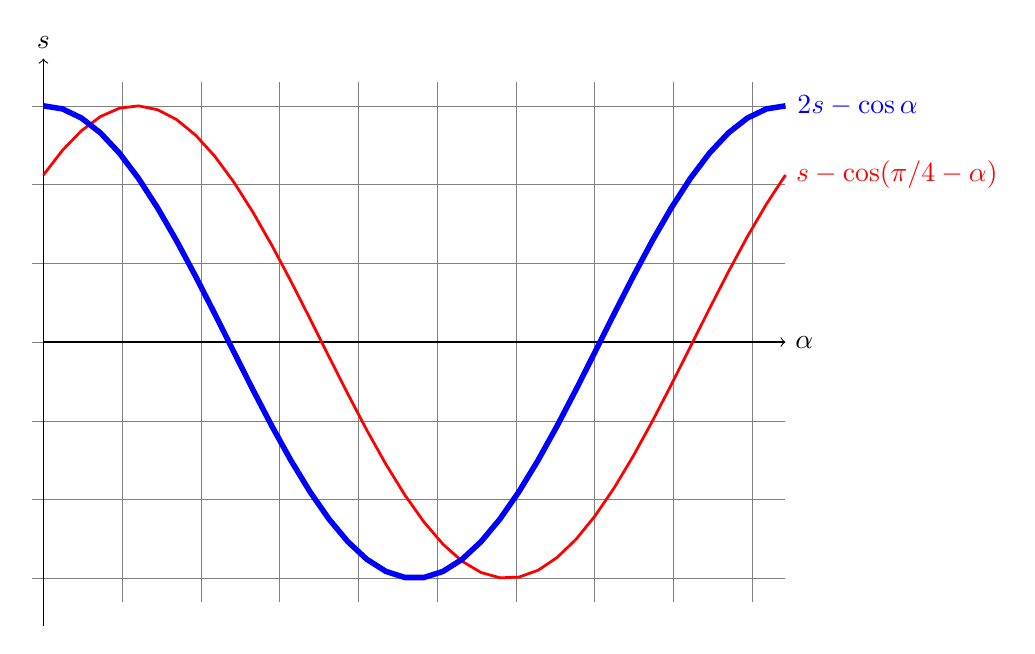
\begin{tikzpicture}[domain=0:2*pi, samples=40, x=1.5cm, y=3cm]
	\draw[very thin,color=gray] (-0.1,-1.1) grid ({2*pi},1.1);
	\draw[->] (0,0) -- (2*pi,0) node[right] {$\alpha$};
	\draw[->] (0,-1.2) -- (0,1.2) node[above] {$s$};
	\draw[color=red, line width=1pt] plot (\x,{cos(pi/4 r-\x r)}) node[right] {$\ddelta{s - \cos(\pi/4 - \alpha)}$};
	\draw[color=blue, line width=2pt] plot (\x,{cos(\x r)}) node[right] {$2\ddelta{s - \cos \alpha}$};
\end{tikzpicture}
\end{document}
